\documentclass{eniepaper}
\卒論
%\修論
\usepackage{epsbox}
\usepackage{makeidx}
\usepackage{fancybox}
\usepackage{subfloat}
\usepackage[dvips]{graphicx}
  \title {Blocklyを用いた多言語対応の\\プログラミング学習支援環境の開発}         
   \author{佐野 裕也}   
   \teacher{香川~考司} 
   \year{平成29年度~(2017年度)}              
\date{平成30年2月15日}                               
% \date{\today}
                                                          
\makeindex                                                
                                         
%\etitle{Development of programming learning support environment for\\ multilingual support using Blockly}
% 2006/2/7改訂
% タイトルを複数行にしたいときは、下のetitleenv環境を使ってください。
\begin{etitleenv}
Development of a Programming Learning Support Environment for Multiple Programming Languages using Blockly
\end{etitleenv}

\begin{eabstract}
When a programming beginner learns a new programming language, he must learn fundamental concepts of  programming and the grammar of the language at the same time. This is a heavy burden him. To solve this, Ozaki  adapted Blockly, a Web-based graphical programming editor, to the C language. In addition, Yamagata  added some special blocks to present exercises to Blockly. In this research, we extend Blockly to further programming languages while keeping the manipulation of the system easy to use. We increase the dynamic deformation of blocks other than the mutator function, so that beginners of programming can expand the range of learning. As a result of evaluation by the students in the laboratory, it was possible to broaden the range of learning of programming beginners by adapting the system to multiple languages, but it was pointed out that the operation is complicated in some situations. In the future, we will improve the system based on the feedback obtained in the laboratory, and confirm the effect in university exercises.
\end{eabstract}

\begin{jabstract}
プログラミング初心者が新たなプログラミング言語を学習するとき、プログラミングの基礎概念と言語の文法を同時に学習しなければならない。 これは、 学習者にとって大きな負担である。これを解決するために尾崎の研究では、WebベースグラフィカルプログラミングエディタであるBlocklyをC言語に対応させた。また山形の研究では、Blocklyに練習問題を提示するためのブロックを実装した。本研究では、システムの操作が容易であることを前提にBlocklyを多言語対応し、Mutator機能以外のブロックの動的変形機能を増やして、プログラミング初心者の学習の幅を広げられるようにした。研究室の学生を対象に評価をした結果、システムの多言語化を行うことでプログラミング初心者の学習の幅を広げることができたが、一部の状況において操作が複雑であることが指摘された。今後は、研究室で得られたフィードバックをもとにシステムを改善し、大学の授業で効果を確認できるようなシステムを目指す。
\end{jabstract}


\begin{keyword}
プログラミング学習, C, JavaScript, Haskell, Flex, Webベース
\end{keyword}

\begin{document} 
\maketitle
%  \listoffigures % 図の目次
%  \listoftables  % 表の目次
                                                          
   \chapter{はじめに}
   
   \section{はじめに}


  プログラミング学習者は、以下の2つを同時に学ばなければならない。
  
\begin{itemize}
\item プログラミングの基礎概念
\item 各プログラミング言語の文法
\end{itemize} 

 これらを学ぶことは、学習者にとって大きな負担である。
 この負担を軽減するために、文法を意識せずにプログラミングができる学習環境が必要である。これを解決するために、Webベースのビジュアルプログラミング言語であるBlockly\cite{Blockly}を用いる。
  
Blocklyとは、Googleで開発されているグラフィカルなプログラミングエディタである。図1のようなブロックを繋ぎ合せることでプログラミングを行う。このため構文エラーに悩まされず、直感的にプログラミングをすることができる。JavaScriptで記述されており、ドキュメントも豊富に用意されているためカスタマイズが容易である。また、BlocklyはWebベースのアプリケーションであるため、導入の作業が不要である。さらに、Blocklyで作成したプログラムは、JavaScript、 Dart、 Python、 Lua、 PHPの5種類のコードに変換して出力することができる。
  
本研究ではBlocklyの多言語化を目標とする。多言語化によって、よりBlocklyで学習支援できる範囲が広がり、学習者が自分に適した言語を選ぶことができる。しかし、必要となるブロックの種類や形状は増加するので、ブロックの形を動的に変形させることも考えなければならない。 


   \section{Webベースの利点}
   
本研究で開発したシステムは、Webベースシステムである。Webベースにすることにより、学習者に次のような利点があると考えられる。

\begin{itemize}
\item システムのインストールが不要
\item Webブラウザがあれば実現可能
\item 常に最新版のシステムが利用可能
\end{itemize} 

また、教員側にも次のような利点がある。

\begin{itemize}
\item システムのカスタマイズが容易
\item システムの不具合をすぐに修正可能
\item 導入に関する指導が不要
\end{itemize} 
 
    \section{先行研究}
    
    \subsection{尾崎の研究}
 
 尾崎の研究\cite{ozaki}は、BlocklyをC言語、Flex言語に対応させたもので、システムの対象者がプログラミング入門者である。このシステムによって文法を意識せずにプログラミンングを学ぶことができる。しかし、大学の講義で学習する言語に対応しきれていない。システム自体が便利であっても、大学の講義で学習する言語に対応していないと、大学生はこのシステムを利用することができない。また、ブロックの形を動的に変形することができないため、柔軟性のあるプログラミング言語をブロックの形状によって制約されてしまうことになる。尾崎の研究で実装したシステムのイメージを図\ref{fig:ozaki}に示す。 


\begin{figure}[h]
\begin{center}
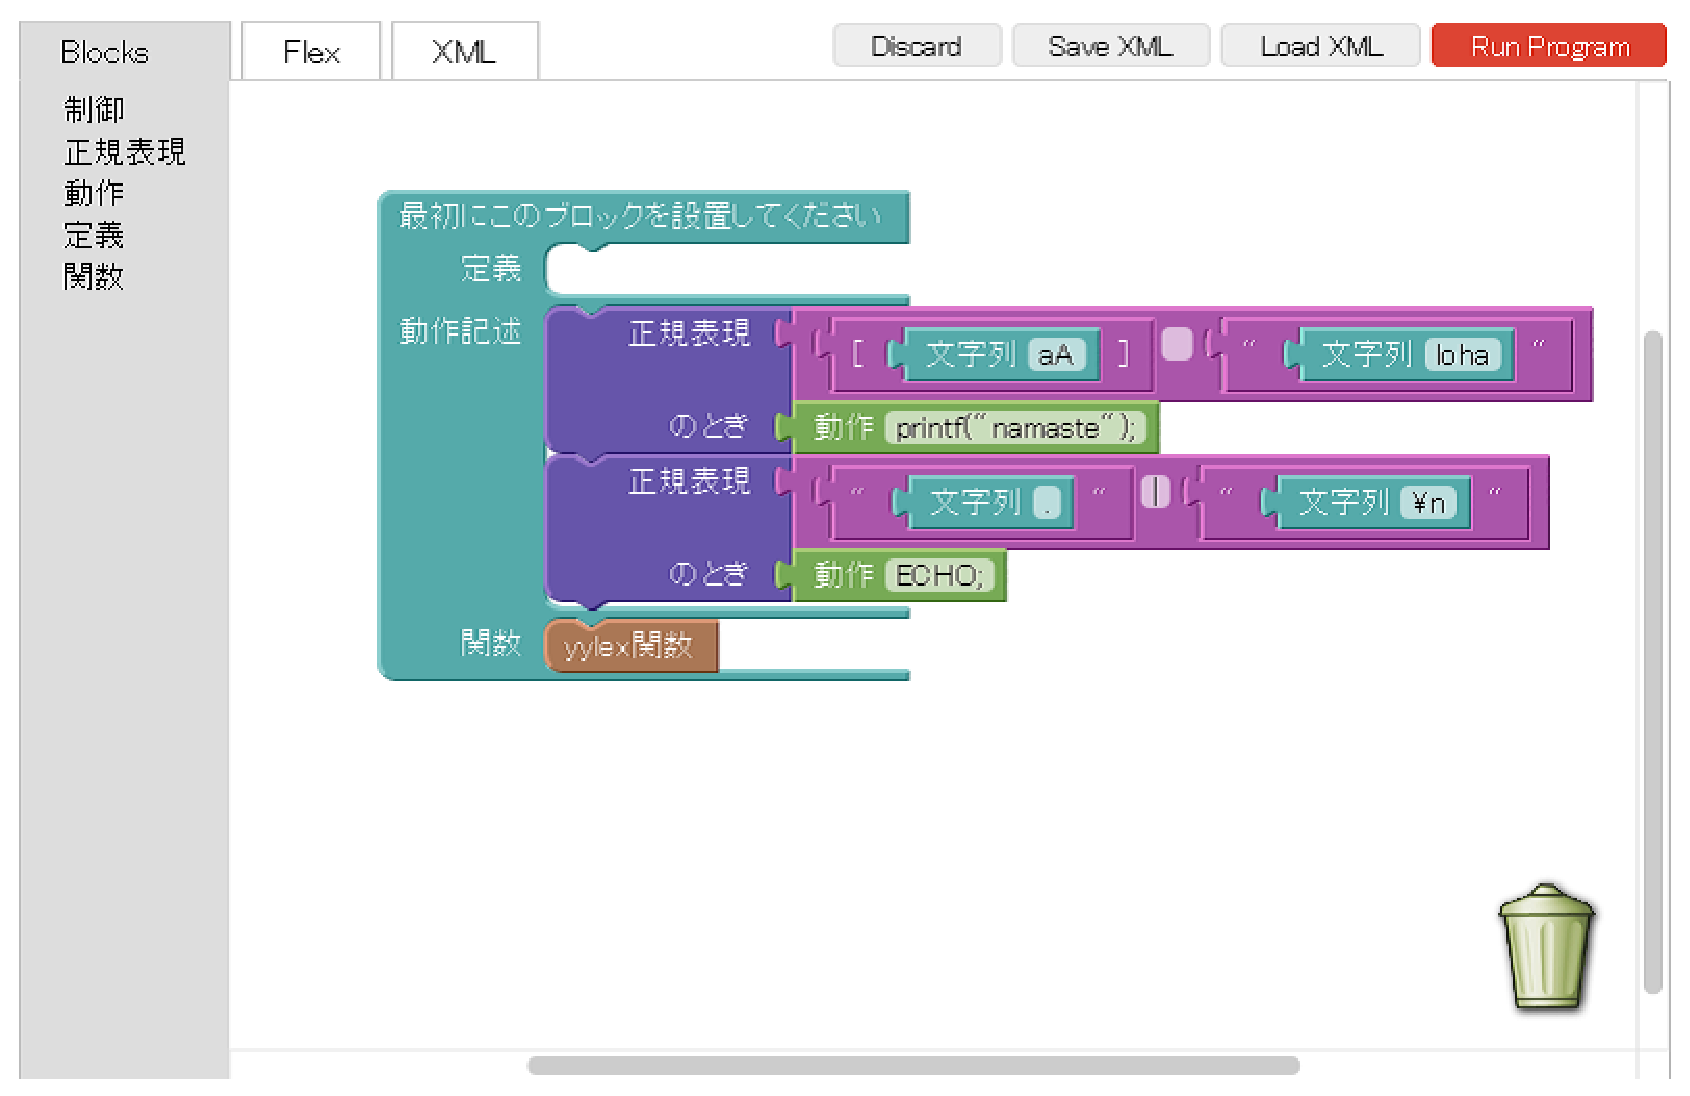
\includegraphics[scale=0.5]{img/ozaki.eps}
\caption{尾崎の研究で実装したシステム}%
\label{fig:ozaki}
\end{center}%
\end{figure}% 
 
	\subsection{山形の研究}
    
 山形の研究\cite{yamagata}は、尾崎の研究でBlocklyをC言語に対応させたものに、問題提示に便利なブロックの追加を行ったものである。このシステムは、ブロックが構文と一対一で対応しており、Blocklyを使った予習の段階から演習の段階まで利用できるようになっている。また、練習問題を選択問題や穴埋め問題だけでなく他の種類の問題も行うことができる。山形の研究で実装したシステムのイメージを図\ref{fig:yamagata}に示す。 
 
\begin{figure}[h]
\begin{center}
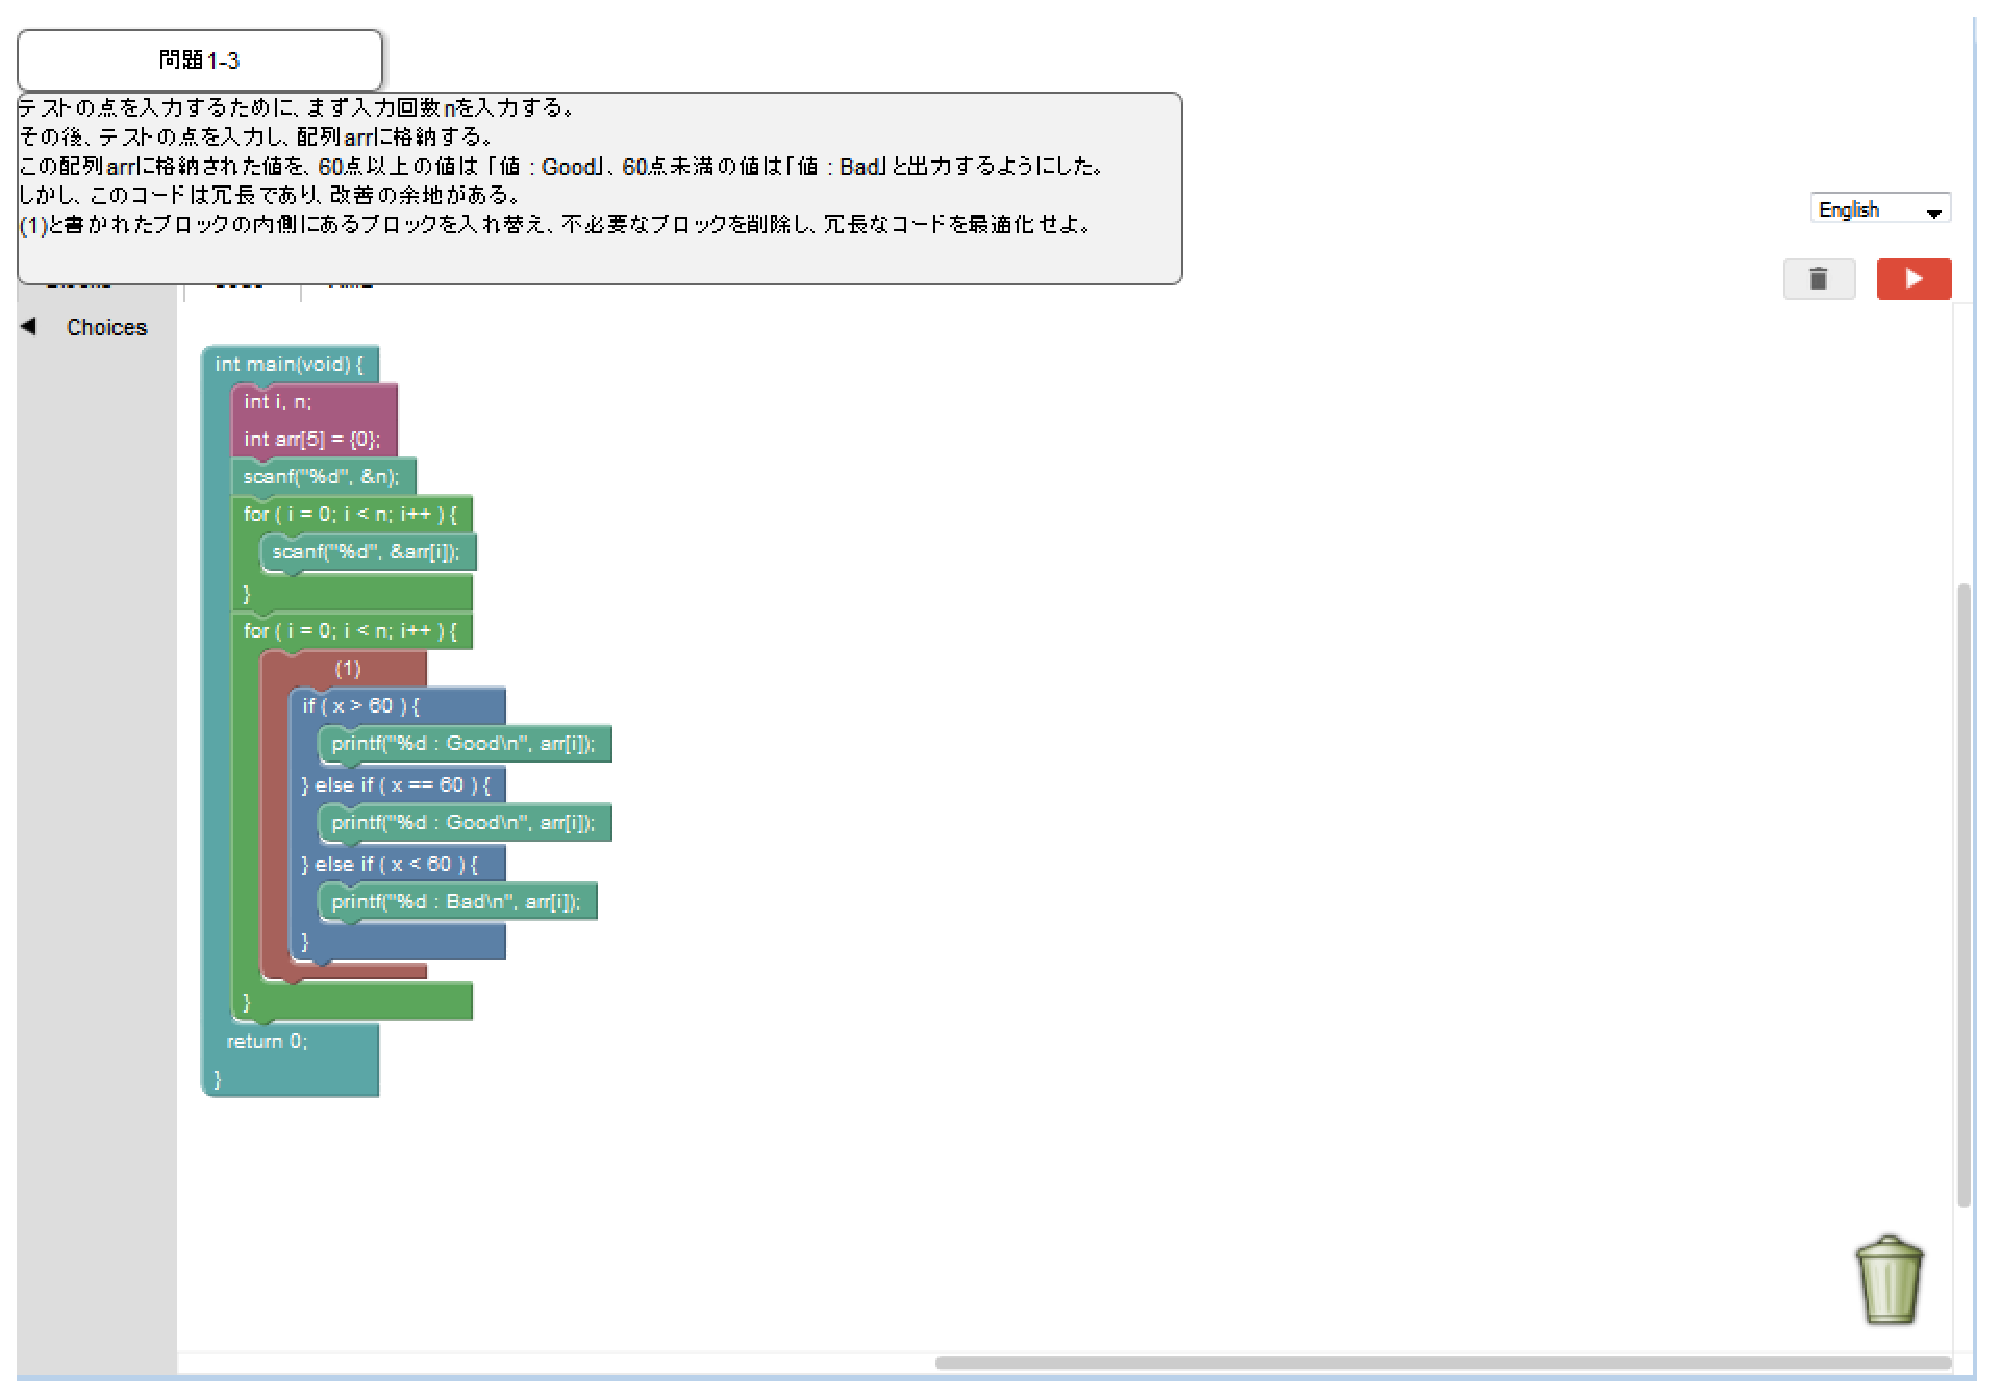
\includegraphics[scale=0.4]{img/yamagata.eps}
\caption{山形の研究で実装したシステム}%
\label{fig:yamagata}
\end{center}%
\end{figure}% 
 
    \section{システムに求められる要件}
    
先行研究の問題点より、本システムに求められる要件は以下の3つである。
 
\begin{itemize}
\item システムの操作が容易
\item 大学の講義で学習する言語に対応させるための多言語化に対応
\item プログラミング言語の柔軟性の保持
\end{itemize} 

大学の講義で学習するプログラミング言語には、C、Java、JavaScript、PHP、Haskell、Flexなどがあるが、いずれの言語もそれぞれの特性を持っており、その特性を踏まえて何も無い状態からソースコードを記述するまで理解するにはかなりの時間と負担がかかる。前の項でも述べた通り、Blocklyはプログラミング入門者に適したシステムなのだが、大学の講義で学習するプログラミング言語に一部対応していない。

これらの問題点を踏まえて、システムの多言語化が必要である。
例えば、関数型言語のHaskellはパターンマッチングを行うが、既存のBlockly for JavaScriptにある関数定義ブロックではこのパターンマッチングに対応しておらず、新たに定義する必要がある。このように、プログラミング言語の文法の違いで新たにブロックを定義する必要があるので、システムの多言語を行うことで必要となるブロックの種類が増加する。
また、柔軟性のあるプログラミング言語をブロックの形状によって制約されてしまう。
これらに対応するために、ブロックの動的変形機能を拡張する。
その際に、プログラミング学習者の負担を軽減させることが目的なので、システムの操作は容易である必要がある。

本論文では、第2章でBlocklyについて、第3章で実装したシステム、第4章でシステムの評価、第5章でまとめ、今後の課題について述べる。



   \chapter{Blockly}
   
   \section{全体の主なファイル構成}
   
Blocklyは、以下のファイルで構成されている。システムに関するファイルのソースコードはJavaScript言語で記述されており、WEBシステムの構成はhtml言語で記述されている。
   
\begin{itemize}

\item core フォルダ

システム自体の定義を行うプログラムで構成されている。
また、blocklyフォルダには、Blocklyの本体であるblockly\_compressed.jsファイルが存在する。

\item demos フォルダ

各システムのWEBページの構成を表すファイルが存在する。
そのほとんどがhtmlで記述されている。

\item blocks フォルダ

このフォルダの直下にブロックの種類ごとのファイルがあり、ブロックの形状を定義している。
これらのプログラムはビルドされ、Libraryフォルダのblocks\_compressed.jsファイルに圧縮されている。
そのため、これらのファイルを書き換えてもシステムが変更されることはない。

\item generators フォルダ

このフォルダの直下に各プログラミング言語のフォルダがある。
それらのフォルダの中にブロックの種類ごとのファイルがあり、各ブロックを配置したときに出力されるソースコードの内容が書かれている。

\item i18n フォルダ

拡張子が.soyのテンプレートがあり、コンパイルすることでJavaScriptファイルを生成する。

\item scripts フォルダ

拡張子が、.shのシェルスクリプトがあり、全体のファイル操作、プログラムの実行内容が記述されている。


\end{itemize} 
  
   \section{システム構成}
   
Blocklyは、ワークスペース部、ブロックメニュー部、ソースコード部、XMLコード部の4つのコンポーネントによって構成される。図\ref{fig:Blockly}にBlocklyのイメージを示す。デフォルトでは、ワークスペース部が表示されており、ソースコードタブを押すとソースコード部のコンポーネントに切り替わり、XMLコードタブを押すとXMLコード部のコンポーネントに切り替わる。ブロックメニュー部は常に左部に表示されている。ここでは、それぞれのコンポーネントについて説明する。
  

\begin{figure}[h]
\begin{center}
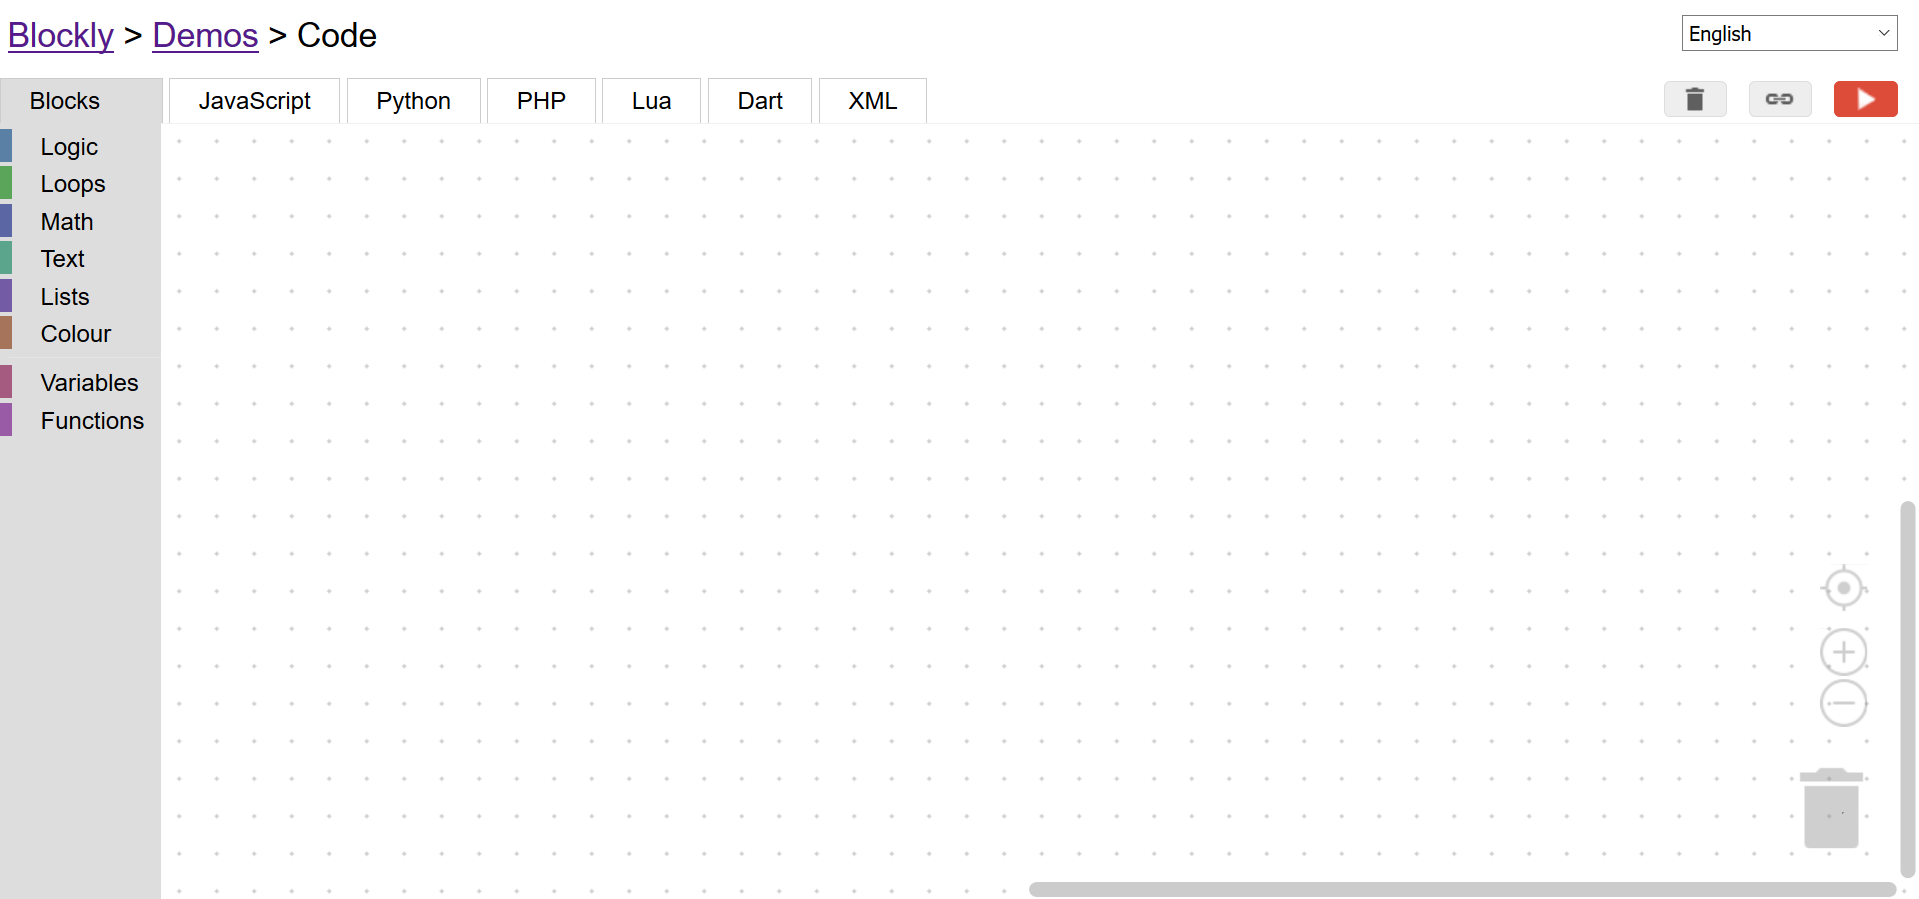
\includegraphics[scale=0.4]{img/Blockly.eps}
\caption{Blockly}%
\label{fig:Blockly}
\end{center}%
\end{figure}% 

   \subsection{ワークスペース部}

ワークスペース部は、ブロックを使ってプログラミングを行うスペースである。図\ref{fig:workspace}にワークスペース部のイメージを示す。ユーザは、ブロック部に存在するブロックをワークスペース部にドラッグ&ドロップで自由につなぎ合わせることでプログラミングを行う。ワークスペース部の右下にはゴミ箱アイコンが存在する。ワークスペース部に設置したブロックをこのアイコンにドラッグすると、ブロックを削除することができる。その上に拡大縮小アイコン、さらにその上に中央に寄せるアイコンが表示されている。

また、ワークスペース部に設置したブロックを右クリックすることで、以下のような動作が行える。

\begin{itemize}
\item ブロックの複製
\item コメントの追加
\item ブロックの接続表現の切り替え
\item ブロックの表現の簡略化
\item ブロックの透明化
\item ブロックの削除
\item ブロックの動作を説明するWebページを表示
\end{itemize} 
   
\begin{figure}[h]
\begin{center}
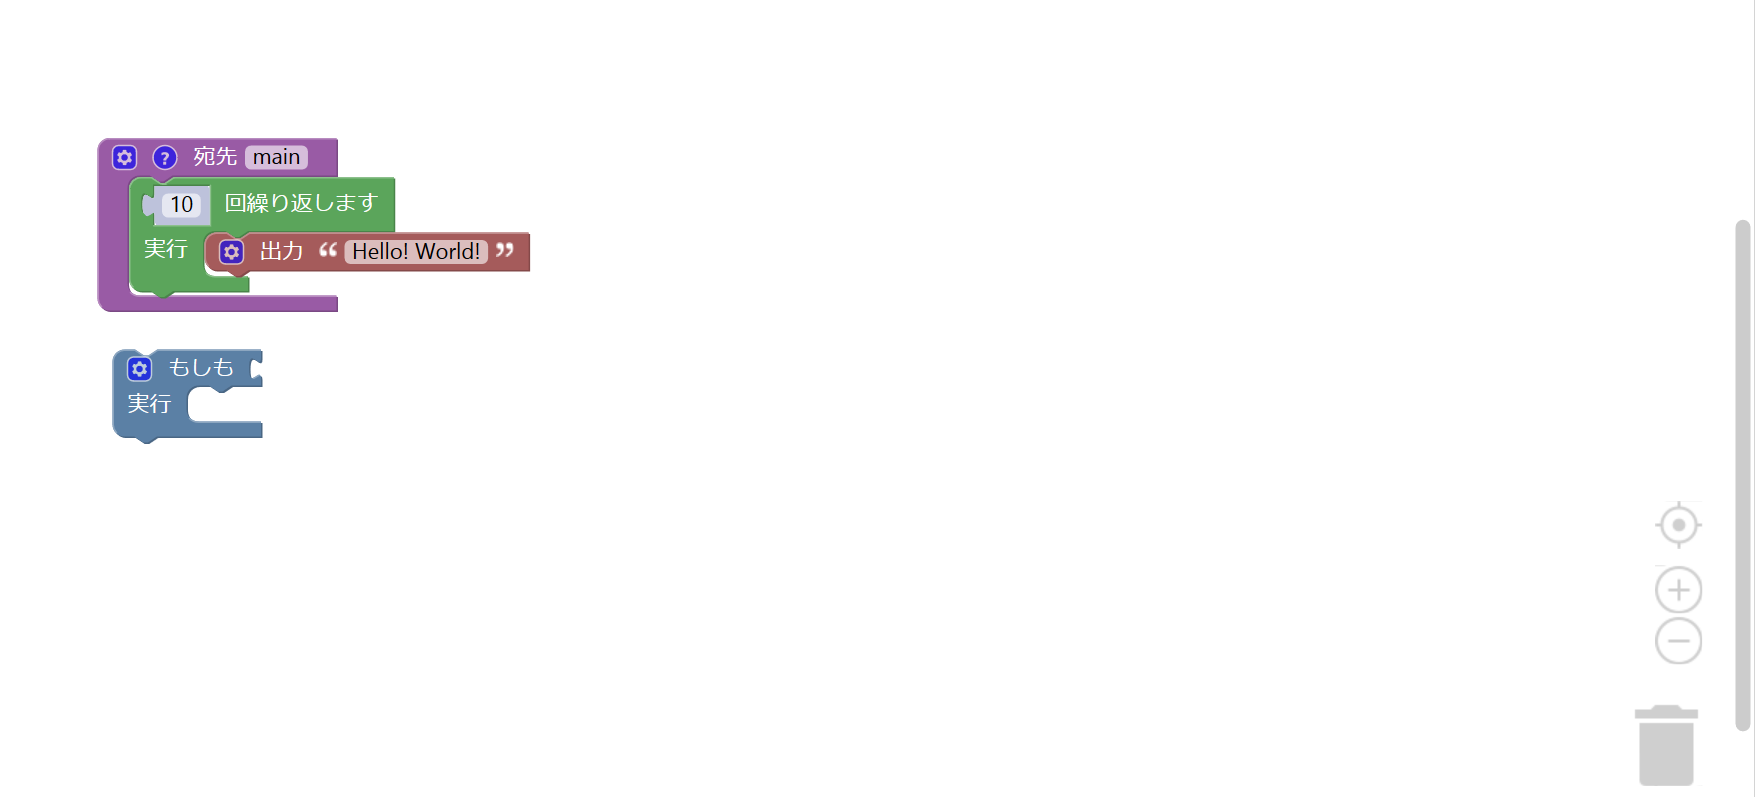
\includegraphics[scale=0.3]{img/workspace.eps}
\caption{ワークスペース部}%
\label{fig:workspace}
\end{center}%
\end{figure}% 

   \subsection{ブロックメニュー部}
   
ブロックメニュー部は、定義されたブロックが存在するスペースである。図\ref{fig:blockmenu}にブロックメニュー部のイメージを示す。ブロックは、論理、数、リストなどのカテゴリーにそれぞれ格納され、カテゴリーをクリックすると、そのカテゴリーに格納されたブロックが表示される。図\ref{fig:blockmenu_open}にカテゴリーをクリックしたときのイメージを示す。ユーザは、このブロックメニューから新たに必要なブロックを選択して使用する。

\begin{figure}[h]
\begin{center}
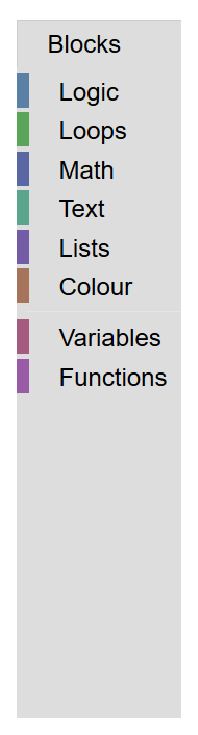
\includegraphics[scale=0.3]{img/blockmenu.eps}
\caption{ブロックメニュー部}%
\label{fig:blockmenu}
\end{center}%
\end{figure}% 

\begin{figure}[h]
\begin{center}
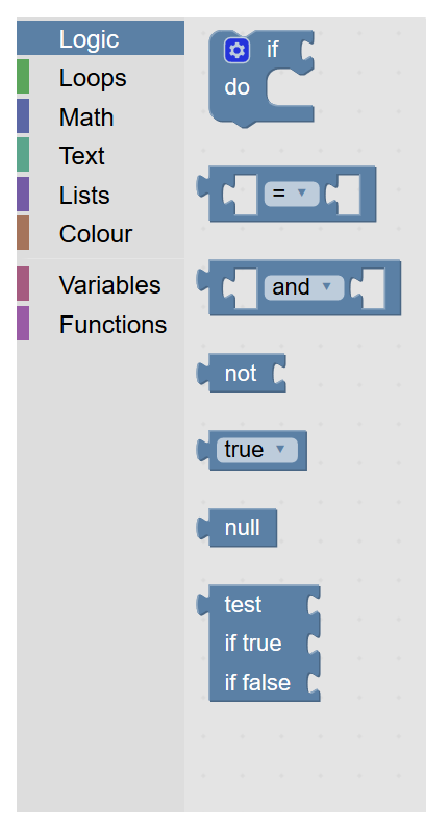
\includegraphics[scale=0.3]{img/blockmenu_open.eps}
\caption{カテゴリーをクリックしたとき}%
\label{fig:blockmenu_open}
\end{center}%
\end{figure}% 

   \subsection{ソースコード部}
   
ソースコード部は、作成したプログラムのソースコードを表示するスペースである。図\ref{fig:source_code}にソースコード部のイメージを示す。タブ名は各プログラミング言語の名称になる。ワークスペース部でブロックを組み合わせて作成したプログラムが、リアルタイムにソースコードに変換され、このソースコード部でいつでも確認することができる。この機能によって、Blocklyでプログラミングを学んだ学習者がソースコードを記述できるように支援する働きを持つ。システムの拡張の際に新たなブロックを実装した場合は、新たなブロックの定義と共に新たにソースコードも定義しなければならない。

\begin{figure}[h]
\begin{center}
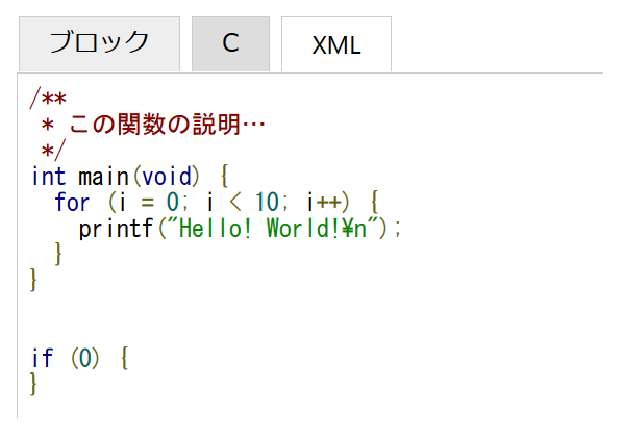
\includegraphics[scale=0.5]{img/source_code.eps}
\caption{ソースコード部}%
\label{fig:source_code}
\end{center}%
\end{figure}% 

   \subsection{XMLコード部}
   
XMLコード部は、作成したプログラムのXMLコードを表示するスペースである。図\ref{fig:XML_code}にXMLコード部のイメージを示す。ワークスペースで組み合わせたブロックの構造がXML形式で出力され、その出力されたXMLコードをセーブ、ロードすることができる。この機能によって、組み合わせたブロックを保存したり、他の学習者や教員が組み合わせたブロックを自分のワークスペース上に再現することができる。以下は、Blocly for C におけるもしも実行ブロックのXMLコードである。blockという要素タグに、type、id、x、y の4つの属性がある。typeの属性値には、ブロックの名前が入り、idの属性値は20文字のランダムな文字列が入り、idは重複しなようになっている。x、y の属性値はワークスペース上の座標が入る。

\shadowbox{
\begin{minipage}[t]{15cm}
\begin{verbatim}
<block type="controls_if" id="RllK?egbl/90CZu2p_wZ" x="-2" y="27"></block>
\end{verbatim}
\end{minipage}
}



\begin{figure}[h]
\begin{center}
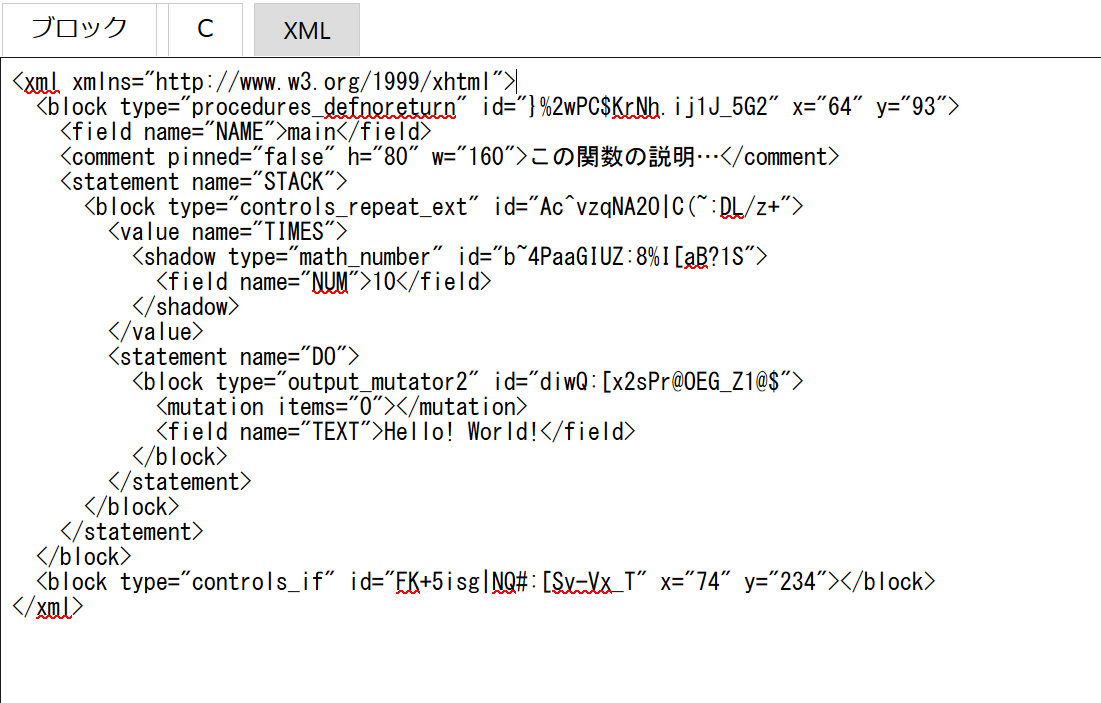
\includegraphics[scale=0.3]{img/XML_code.eps}
\caption{XMLコード部}%
\label{fig:XML_code}
\end{center}%
\end{figure}% 
   
   \section{オプション機能}
   
Blocklyには、オプション機能がある。以下の図\ref{fig:blockly_option}にオプション機能のイメージを示す。これは、システムWEBページの右下にあるものである。図には4つのアイコンがあり、上から、中央に寄せる、拡大、縮小、削除である。

\begin{itemize}

\item 中央に寄せるアイコン

このアイコンは、ワークスペース部で組み立てたプログラムを中央に寄せることができる機能である。

\item 拡大・縮小アイコン

拡大・縮小アイコンは、組み立てたプログラム全体を拡大・縮小することができる機能である。大規模なプログラミングを組み立てるときになくてはならない機能である。

\item 削除アイコン

削除アイコンは、ワークスペース部にあるブロックを削除できる機能である。操作方法として、削除したいブロックをドラッグして削除アイコン上でドロップすることで削除できる。また、同様の機能として、削除したいブロック上で右クリックした際のコンテクストメニューにも削除がある。

\end{itemize} 

\begin{figure}[h]
\begin{center}

\includegraphics[scale=0.5]{img/blockly_option.eps}
\caption{オプション機能}%
\label{fig:blockly_option}
\end{center}%
\end{figure}% 


   \section{Mutator機能}
   
Blocklyの機能にMutatorがある。ここでは、そのMutatorという機能について説明する。

Mutatorは、ブロックの動的変形を行う機能である。この機能は、Blocklyが用意している機能の中で唯一の動的変形である。図\ref{fig:mutator1}にMutatorのイメージを示す。Mutatorの機能が使えるブロックには、左上に歯車がある場合がある。その歯車のマークを押すと、その近くに吹き出しの形をした小窓が現れる。小窓の左半分はブロックメニュー部、右半分はワークスペース部となっている。小窓の中のコンポーネントは、このブロック限定のものである。小窓のブロックメニュー部から拡張したいブロックを取り出し、小窓のワークスペース部の既存のブロックに取り付ける。すると、吹き出し元のブロックが変形される。図\ref{fig:mutator2}が、そのときのイメージである。Mutator機能によって、ブロックの形をカスタマイズでき、ブロックメニュー部で用意されるブロックの種類を大幅に減らすことができる。実装で動的変形機能の拡張を行うときは、この機能を参考にして新たな動的変形機能を実装する。

\begin{figure}[h]
\begin{center}
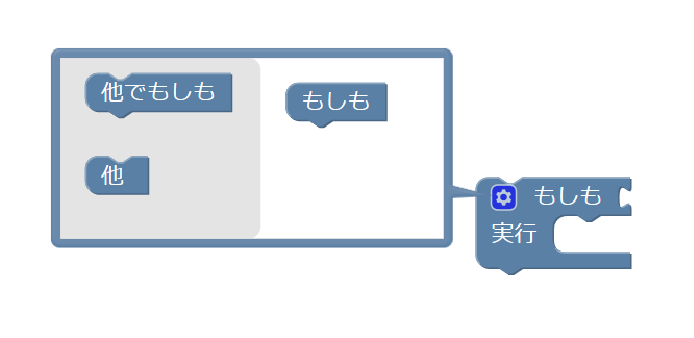
\includegraphics[scale=0.5]{img/mutator1.eps}
\caption{動的変形前のMutatorブロック}%
\label{fig:mutator1}
\end{center}%
\end{figure}% 

\begin{figure}[h]
\begin{center}
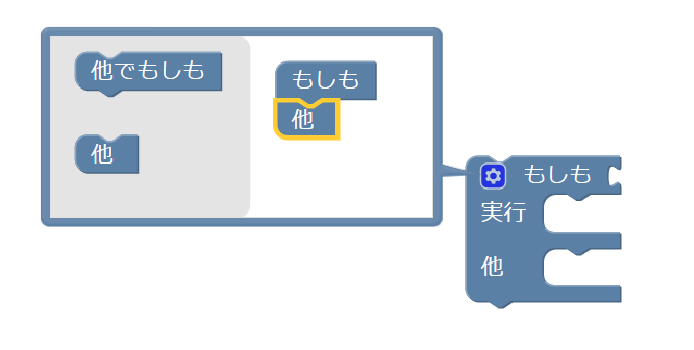
\includegraphics[scale=0.5]{img/mutator2.eps}
\caption{動的変形後のMutatorブロック}%
\label{fig:mutator2}
\end{center}%
\end{figure}% 

   \section{ブロックの定義}
   
ここで、ブロックの定義方法について述べる。
まず初めに、一般的なブロック定義のソースコードを以下に示す。
ブロックの形状を定義したいときは、init関数のなかに関数を記述していく。

\shadowbox{
\begin{minipage}[t]{15cm}
\begin{verbatim}
Blockly.Blocks['sample_name'] = {
  init: function() {
    this.setColour(100);
    this.appendDummyInput().appendField("サンプル");
    this.setPreviousStatement(true);
    this.setNextStatement(true);
    this.setOutput(true, 'String');
    this.appendValueInput('A');
    this.setInputsInline(true);
    this.appendStatementInput('DO0');
    this.setTooltip("このブロックは、サンプルです。");
  }
};
\end{verbatim}
\end{minipage}
}

Blocklyには新たなブロックを定義するためにいくつかの関数が用意されている。以下にそれぞれの関数の機能と使用方法を示す。

\begin{itemize}

\item appendField

appendFieldは、ブロック上に文字列や入力フォーム、ドロップダウンメニューを定義する関数である。この関数の前にappendDummyInput関数を呼び出す必要がある。
以下は、appendFieldの使用例である。

\shadowbox{
\begin{minipage}[t]{14cm}
\begin{verbatim}
this.appendDummyInput().appendField("サンプル");
\end{verbatim}
\end{minipage}
}

\item setColor

setColorは、ブロックの色を定義する関数である。0から360までにの数値を指定することで、ブロックの色を定義することができる。
以下は、setColorの使用例である。

\shadowbox{
\begin{minipage}[t]{8cm}
\begin{verbatim}
this.setColour(100);
\end{verbatim}
\end{minipage}
}

\item setPreviousStatement

setPreviousStatementは、ブロック上接続部の有無を定義する関数である。第1引数がtrueなら接続部が有りで、falseなら無しである。
以下は、setPreviousStatementの使用例である。

\shadowbox{
\begin{minipage}[t]{8cm}
\begin{verbatim}
this.setPreviousStatement(true);
\end{verbatim}
\end{minipage}
}

\item setNextStatement

setNextStatementは、ブロック下接続部の有無を定義する関数である。この関数も同様に、第1引数がtrueなら接続部が有りで、falseなら無しである。
以下は、setNextStatementの使用例である。

\shadowbox{
\begin{minipage}[t]{8cm}
\begin{verbatim}
this.setNextStatement(true);
\end{verbatim}
\end{minipage}
}

\item setOutput

setOutputは、ブロック左接続部の有無を定義する関数である。第1引数がtrueなら接続部が有りで、falseなら無しである。第2引数は、接続先のブロック型を指定する。接続先のブロックの型が指定したものと同じならブロックを接続することができる。型の指定がない場合は、第2引数ごと無くすか、nullを指定する。
以下は、setOutputの使用例である。

\shadowbox{
\begin{minipage}[t]{8cm}
\begin{verbatim}
this.setOutput(true, 'String');
\end{verbatim}
\end{minipage}
}

\item appendValueInput

appendValueInputは、ブロック右接続部の有無を定義する関数である。この接続部に関する関数は、1つのブロックに対し複数指定できる。第1引数には、接続部の名称を指定できる。接続部の名称を指定することで、ブロックの他の接続部と区別させるためである。一般には、変数ブロックや数ブロックを接続する。setCheck関数をそのあとにつけることで接続先のブロックの型を指定できる。
以下は、appendValueInputの使用例である。

\shadowbox{
\begin{minipage}[t]{14cm}
\begin{verbatim}
this.appendValueInput('A').setCheck('int');
\end{verbatim}
\end{minipage}
}

\item setInputsInline

setInputsInlineは、appendValueInput関数で定義した右接続部をブロックの内側(以後ソケットと呼ぶ)にするかを定義する関数である。第1引数がtrueならソケットとして定義し、falseなら右接続部そのままである。
以下は、setInputsInlineの使用例である。

\shadowbox{
\begin{minipage}[t]{8cm}
\begin{verbatim}
this.setInputsInline(true);
\end{verbatim}
\end{minipage}
}

\item appendStatementInput

appendStatementInputは、ブロックの内側で上接続部を定義したブロックと接続できるように定義する関数である。第1引数には、接続部の名称を指定できる。接続部の名称を指定することで、ブロックの他の接続部と区別させるためである。一般には、命令ブロックと接続する。
以下は、appendStatementInputの使用例である。

\shadowbox{
\begin{minipage}[t]{8cm}
\begin{verbatim}
this.appendStatementInput('DO');
\end{verbatim}
\end{minipage}
}

\item setTooltip

setTooltipは、ブロック上にカーソルを合わせたときに表示される内容を定義する関数である。第1引数は、表示する内容を文字列で定義する。
以下は、setTooltipの使用例である。

\shadowbox{
\begin{minipage}[t]{8cm}
\begin{verbatim}
this.setTooltip("このブロックは、サンプルです。");
\end{verbatim}
\end{minipage}
}

\end{itemize} 

   \chapter{実装}
   
本研究では、Blocklyで多言語化を行うために、以下のような実装を行った。
   
   \section{多言語化}
   
   \subsection{対応する言語の種類}
   
まず、Blocklyの多言語化を行うために、対応するプログラミング言語の種類を決めなければならない。講義で学ぶプログラミング言語から考えて本システムでは、4種類のプログラミング言語に対応できるようにした。それが以下の4種類のシステムである。

\begin{itemize}
\item Blockly for C

先行研究で尾崎と山形が開発したシステムを引き継いで実装を行った。

\item Blockly for JavaScript

Bloclyの既存のシステムに用意された言語である。

\item Blockly for Haskell

Haskell[4]言語は、本研究であらたに導入される言語である。Blocklyの既存に対応している言語と先行研究で実装されている言語はいずれも命令型プログラミング言語であるが、Haskellは宣言型プログラミング言語である。Blocklyに宣言型プログラミング言語を導入してはどうかということで、Blocklyにあらたに導入される言語として決定した。

\item Blockly for Flex

先行研究で尾崎が開発したシステムを引き継いで実装を行った。特に、正規表現ブロックの一部を改良した。

\end{itemize} 
   
   \subsection{システムのWEBページ}
   
Blocklyの既存のシステムでは、1つのWEBページでBlocklyの対応する言語をサポートしている。1つのWEBページに対応言語名が書かれた複数のソースコードタブが存在し、ワークスペースでブロックを組み立てた後に、ソースコードを表示したい言語のタブを押してソースコードを確認するようになっている。しかし、どのソースコードタブを押してもブロックカテゴリーはすべて同じなので、Blocklyに対応するすべての言語に共通できるブロックしか作成することができない。

本システムでは、多言語化を行うために1種類の言語に、1つのWEBページを用意した。また、筆者が開発したWEBページにスムーズにアクセスできるように、それぞれの言語のシステムのリンク先を貼り付けたデモページの索引ページも作成した。索引ページのイメージが図\ref{fig:index}である。

\begin{figure}[h]
\begin{center}
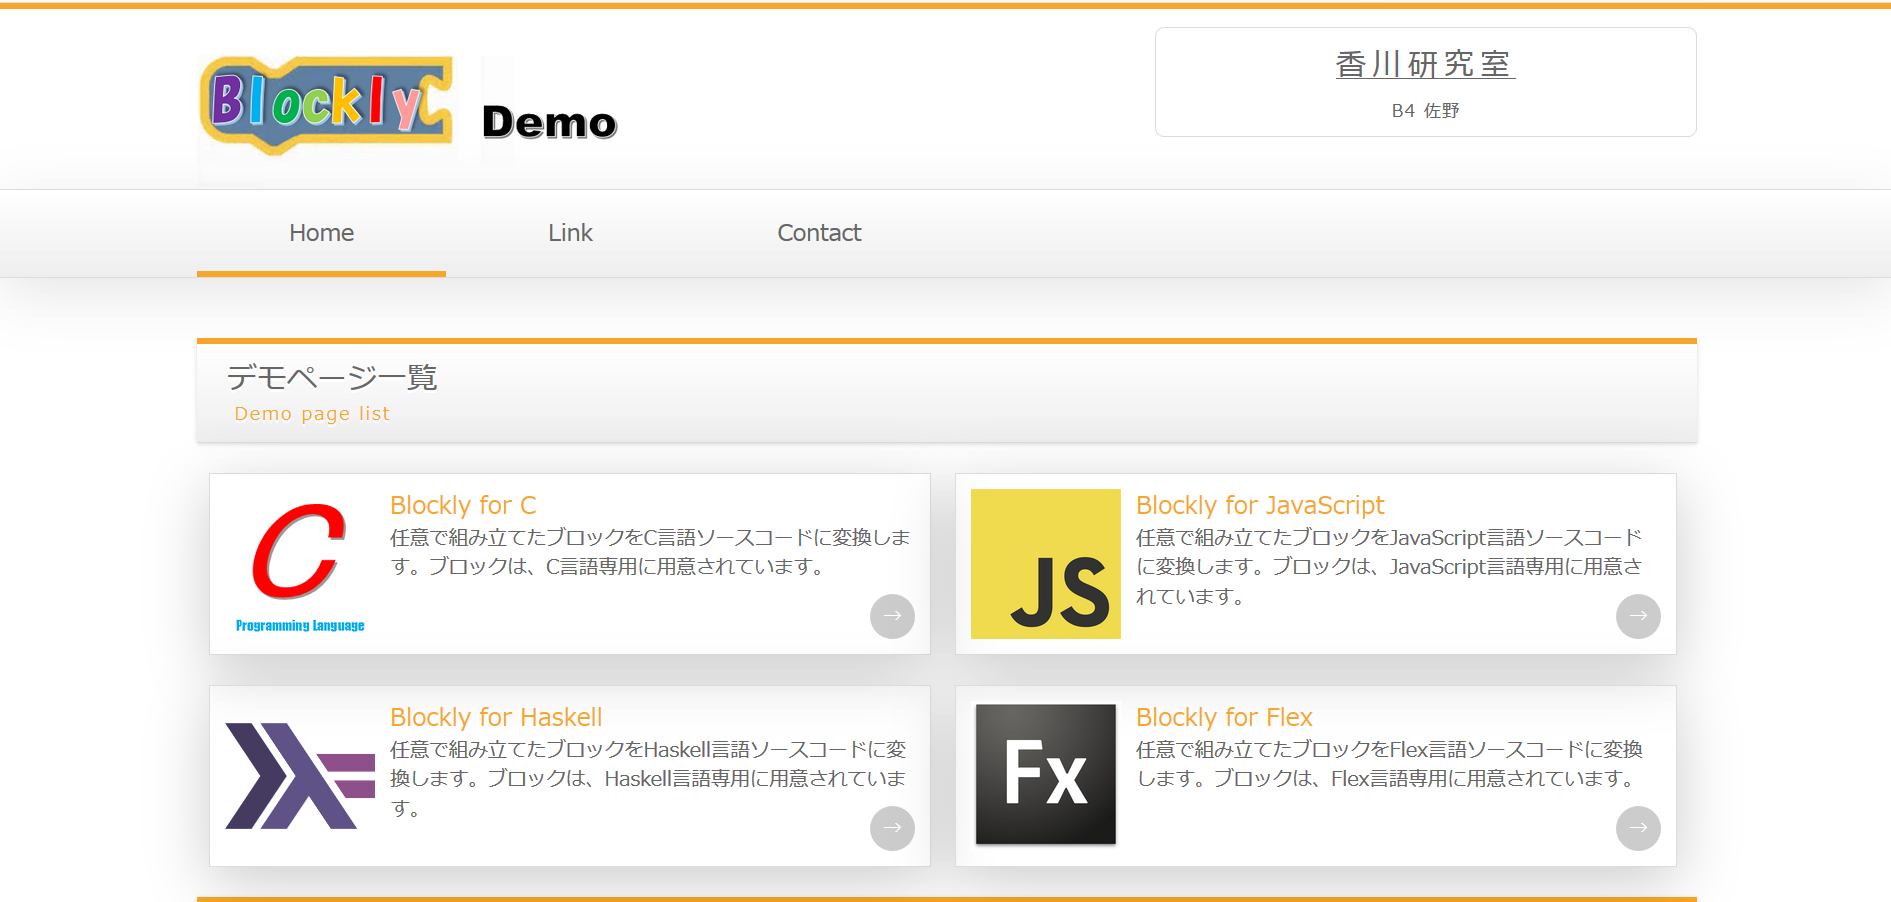
\includegraphics[scale=0.5]{img/index.eps}
\caption{索引ページ}%
\label{fig:index}
\end{center}%
\end{figure}% 

   \section{動的変形機能}
   
Mutatorは、Blocklyの既存に用意されている機能だが、本システムで新たに実装した動的変形機能を具体的なブロックを例に挙げて説明する。

本システムで新たに開発した動的変形機能は、printfブロックに実装されている。そのブロックのイメージは、図\ref{fig:output}である。このブロックは、Blockly for C で用意されている。Mutator機能では、ブロックの左上に歯車マークがあり動的変形機能が実装されていることが分かるが、このブロックは歯車マークの代わりになるものがないので、動的変形機能が実装されていることが分からない。しかし、このブロックの入力フォームに図\ref{fig:output2}のような文字列を入力すると、動的変形機能が実装されていることが分かる。これは、入力フォームで"\%"の数を検出して、その数だけソケットの数を動的変形機能で増やしている。ソケットとは、変数ブロックや数ブロックを挿入できる穴である。検出のタイミングは、入力フォームの中身に変化があるごとに行われる。この機能は、いちいち歯車マークをクリックして別途でブロックを組み立てる必要もないので、動的変形の手間を省きかつ操作もシンプルになっているので、プログラミング学習者の負担を軽減させることができている。

\begin{figure}[h]
\begin{center}

\includegraphics[scale=0.5]{img/output.eps}
\caption{動的変形前のprintfブロック}%
\label{fig:output}
\end{center}%
\end{figure}% 

\begin{figure}[h]
\begin{center}

\includegraphics[scale=0.5]{img/output2.eps}
\caption{動的変形後のprintfブロック}%
\label{fig:output2}
\end{center}%
\end{figure}% 
   
   \section{新たに作成したブロック}

ここでは、本システムで新たに実装したブロックについて分類ごとに分けて説明する。
   
   \subsection{Blockly for C}

本小節では、Blockly for C で新たに実装したブロックについて説明する。

\begin{itemize}

\item 入力・出力ブロック

プログラムにおける入力、出力の処理を表すブロックである。ブロックカテゴリーに格納されている状態では入力フォームのみだが、動的変形機能によって入力フォームに入力された"\%"の数を自動検出してソケットを増やしていく。以下の図\ref{fig:inoutput}に、入力・出力ブロックを示す。

\begin{figure}[h]
\begin{center}

\includegraphics[scale=0.5]{img/inoutput.eps}
\caption{入力・出力ブロック}%
\label{fig:inoutput}
\end{center}%
\end{figure}% 

\item ヘッダブロック群

C言語のヘッダファイルを表すブロック群である。Blockly for C のブロックカテゴリーのヘッダに格納されている。以下の図\ref{fig:header}に、ヘッダブロック群を示す。

\begin{figure}[h]
\begin{center}
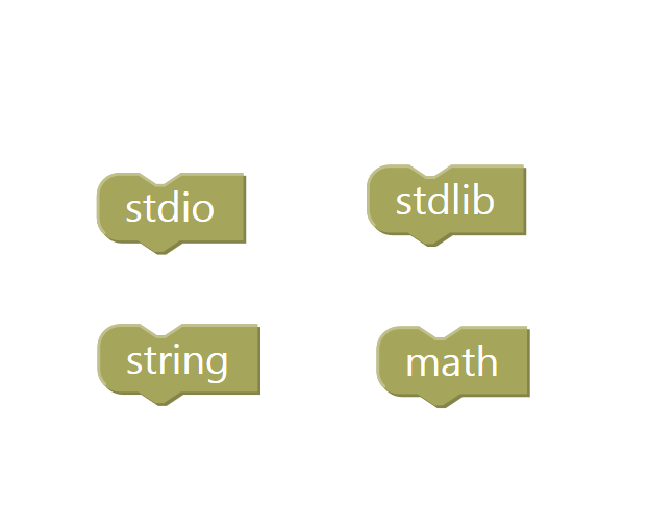
\includegraphics[scale=0.5]{img/header.eps}
\caption{ヘッダブロック群}%
\label{fig:header}
\end{center}%
\end{figure}% 

\end{itemize} 
   
   \subsection{Blockly for Flex}

本小節では、Blockly for Flex で表現できる文法を先に説明し、その後に新たに実装したブロックについて説明する。

\begin{itemize}

\item Blockly で表現できる正規表現の範囲

- 文字列そのものを表す。以下の表記が記述例である。abc+という4文字を表している。

\shadowbox{
\begin{minipage}[t]{3cm}
\begin{verbatim}
”abc+”
\end{verbatim}
\end{minipage}
}

- 特殊文字を文字そのものにする。以下の表記が記述例である。* という特殊文字を文字化してる。

\shadowbox{
\begin{minipage}[t]{3cm}
\begin{verbatim}
\*
\end{verbatim}
\end{minipage}
}

- 文字の集合を表現する。以下の表記が記述例である。aまたはbまたはcの1文字を表している。

\shadowbox{
\begin{minipage}[t]{3cm}
\begin{verbatim}
[abc]
\end{verbatim}
\end{minipage}
}

- 文字集合の範囲を指定する。以下の表記が記述例である。0から9までの1文字を表している。

\shadowbox{
\begin{minipage}[t]{3cm}
\begin{verbatim}
[0-9]
\end{verbatim}
\end{minipage}
}

- 補集合を指定する。以下の表記が記述例である。数字位階の1文字を表している。

\shadowbox{
\begin{minipage}[t]{3cm}
\begin{verbatim}
[^0-9]
\end{verbatim}
\end{minipage}
}

- 改行を除く任意の文字を表現する。以下の表記が記述例である。

\shadowbox{
\begin{minipage}[t]{3cm}
\begin{verbatim}
.
\end{verbatim}
\end{minipage}
}

- 二者択一を表現する。以下の表記が記述例である。aまたはbの1文字を表している。

\shadowbox{
\begin{minipage}[t]{3cm}
\begin{verbatim}
a|b
\end{verbatim}
\end{minipage}
}

- 選択の任意を表現する。以下の表記が記述例である。abまたはaを表している。

\shadowbox{
\begin{minipage}[t]{3cm}
\begin{verbatim}
ab?
\end{verbatim}
\end{minipage}
}

- 0個以上の繰り返しを表現する。以下の表記が記述例である。aの0個以上の繰り返しを表している。

\shadowbox{
\begin{minipage}[t]{3cm}
\begin{verbatim}
a*
\end{verbatim}
\end{minipage}
}

- 1個以上の繰り返しを表現する。以下の表記が記述例である。aの1個以上の繰り返しを表している。

\shadowbox{
\begin{minipage}[t]{3cm}
\begin{verbatim}
a+
\end{verbatim}
\end{minipage}
}

\item 正規表現のブロック群

Blockly for Flex では、先行研究で尾崎が実装したブロックを参考にしながら正規表現のブロックを一新した。ソケットを使うことで、複数の文字範囲を正規表現で表せるようになっているが、2個が限界である。動的変形機能を使って3個以上の文字範囲が実装できるように開発中である。ブロックの表現は、実際のFlexの文法の記述形式としている。これでユーザは、構文エラーに悩まされることなくプログラミングを行うことができる。以下の図\ref{fig:flex_RE_blocks}に、正規表現のブロック群を示す。

\begin{figure}[h]
\begin{center}

\includegraphics[scale=0.5]{img/flex_RE_blocks.eps}
\caption{正規表現ブロック群}%
\label{fig:flex_RE_blocks}
\end{center}%
\end{figure}% 

\end{itemize} 

   \subsection{Blockly for Haskell}
   
本小節では、Blockly for Haskell で新たに実装したブロックについて説明する。Haskellでは、関数におけるパターンマッチングによる場合分けで処理を定義することができ、引数がリストの場合にも対応した。また、内包表記を扱ったリストもブロックで表現可能である。

\begin{itemize}

\item もしも実行ブロック

もしも実行ブロックは、他の言語のシステムでも既存に用意されてるブロックだが、Blockly for Haskellでは、Haskellの文法の性質上、違うので新たに用意した。また、“if then else”文の“then”と“else”のあとには、式がくるので、ブロックのつなぎ目の形を変形させた。以下の図\ref{fig:haskell_if}に、Blockly for Haskell で新に実装したもしも実行ブロックを示す。

\begin{figure}[h]
\begin{center}

\includegraphics[scale=0.5]{img/haskell_if.eps}
\caption{もしも実行ブロック}%
\label{fig:haskell_if}
\end{center}%
\end{figure}% 

\item 制御ブロック群

Blockly for Haskellでブロックカテゴリーの制御で新たにブロックを実装した。mainブロック、doブロック、letブロックである。以下の図\ref{fig:haskell_logic}に、Blockly for Haskellの実装した制御ブロック群を示す。

\begin{figure}[h]
\begin{center}

\includegraphics[scale=0.5]{img/haskell_logic.eps}
\caption{Haskellの制御ブロック群}%
\label{fig:haskell_logic}
\end{center}%
\end{figure}% 

\item リスト内包表記ブロック

Blockly for Haskell のリストカテゴリーで新たに内包表記ブロックを実装した。以下の図\ref{fig:inner_table}に、内包表記ブロックを示す。図の左が、リスト内包表記ブロックに何も接続していない初期状態で、右がリスト内包表記ブロックの接続例である。リスト内包表記のソースコードは、リストの中に1つの式と複数の限定式で記述される。リスト内包表記ブロックでは、内包表記と書かれた右のソケットに式を挿入式し、限定式と書かれたところの右に複数の限定式を表すブロックを挿入する仕様となっている。

\shadowbox{
\begin{minipage}[t]{6cm}
\begin{verbatim}
[ 式 | 限定式, ... , 限定式 ]
\end{verbatim}
\end{minipage}
}

\begin{figure}[h]
\begin{center}
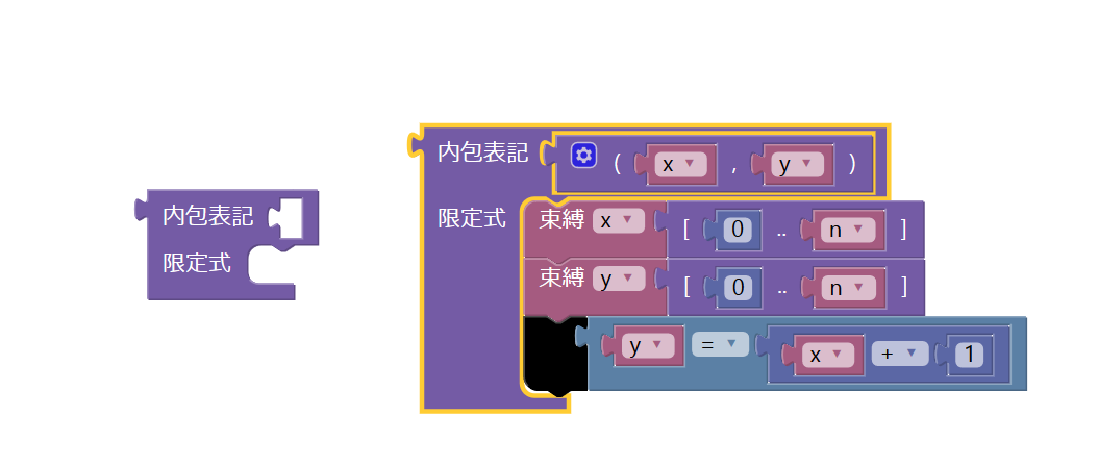
\includegraphics[scale=0.5]{img/inner_table.eps}
\caption{リスト内包表記ブロック}%
\label{fig:inner_table}
\end{center}%
\end{figure}% 

\item 関数定義ブロック

Blockly for Haskell で新たに関数定義ブロックを実装した。以下の図\ref{fig:haskell_function1}に、関数定義ブロックの何も接続していない初期状態と関数定義ブロックの小窓の中身を示す。関数定義ブロックでは、Mutator機能でブロックを動的に変形させることができる。このMutator機能で関数の仮引数を自由に設定することができ、小窓のなかの型ブロックを引数コンテナに組み立てることで仮引数を調整できる。また、引数コンテナに接続された一番下の型ブロックは、関数定義ブロックの返却値となり、関数定義ブロックを動的変形に変形しない仕様となっている。

1つの関数定義ブロックで1つのパターンマッチングができるようになっており、仮引数の型が書かれている接続部に仮引数のパターンの変数ブロックやリストブロックを接続する。それらの下の式と書かれた接続部にパターンに対応した式ブロックを接続する。

\begin{figure}[h]
\begin{center}
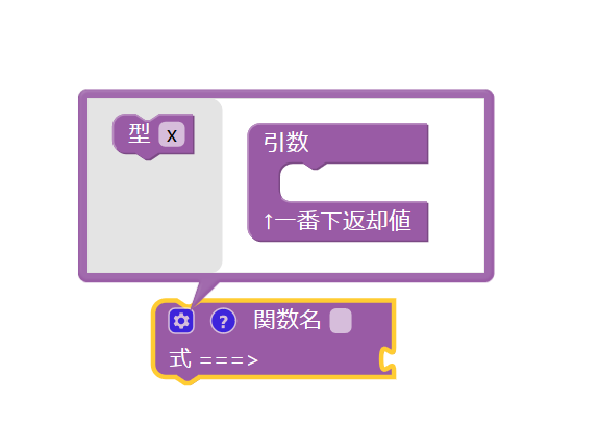
\includegraphics[scale=0.5]{img/haskell_function1.eps}
\caption{関数定義ブロックの初期状態と小窓の中身}%
\label{fig:haskell_function1}
\end{center}%
\end{figure}% 

\item 関数呼び出しブロック

関数呼び出しブロックは、関数ブロックを右クリックしてコンテクストメニューで取り出すことができる。このブロックのソケットは、実引数を表し変数ブロックや数ブロックを挿入する。関数呼び出しブロックは、ブロックカテゴリー部にはない唯一のブロックである。関数定義ブロックの仮引数の数と関数呼び出しブロックの実引数のソケットの数は動的に対応できるようになっている。以下の図\ref{fig:haskell_function_call}に関数呼び出しブロックを示す。

\begin{figure}[h]
\begin{center}

\includegraphics[scale=0.5]{img/haskell_function_call.eps}
\caption{関数呼び出しブロック}%
\label{fig:haskell_function_call}
\end{center}%
\end{figure}% 

\item 関数定義ブロックと関数呼び出しブロックの接続例

以下の図\ref{fig:haskell_function2}に、関数定義ブロックと関数呼び出しブロックの接続例を示す。図の関数定義ブロックでは、小窓のなかの引数コンテナに型ブロックが3個接続されている。そして、本体の関数定義ブロックには、仮引数の接続部が2か所ある。これは、小窓のなかの引数コンテナに接続されている一番下の型ブロックが、関数の返却値を示しているためである。

今回の例のパターンマッチングでは、第1仮引数は任意の変数で、第2仮引数は任意のリストである。その際のリストの先頭要素をx、それ以降のリストをxsを表す。式と書かれた接続部では、もしも実行ブロックを接続し、もしも任意の変数nとリストの先頭要素xが等しければリストxsを返し、それ以外なら先頭要素がxでそれ以降の要素は関数deleteOneを呼び出したリストを返す。リストの中で呼び出した関数deleteOneの第1実引数はn、第2実引数はxsである。

このブロック状態でのソースコードは以下のようになっている。

\shadowbox{
\begin{minipage}[t]{15cm}
\begin{verbatim}
deleteOne n (x:xs) = if n == x then xs else (x:deleteOne n xs)
\end{verbatim}
\end{minipage}
}

\begin{figure}[h]
\begin{center}
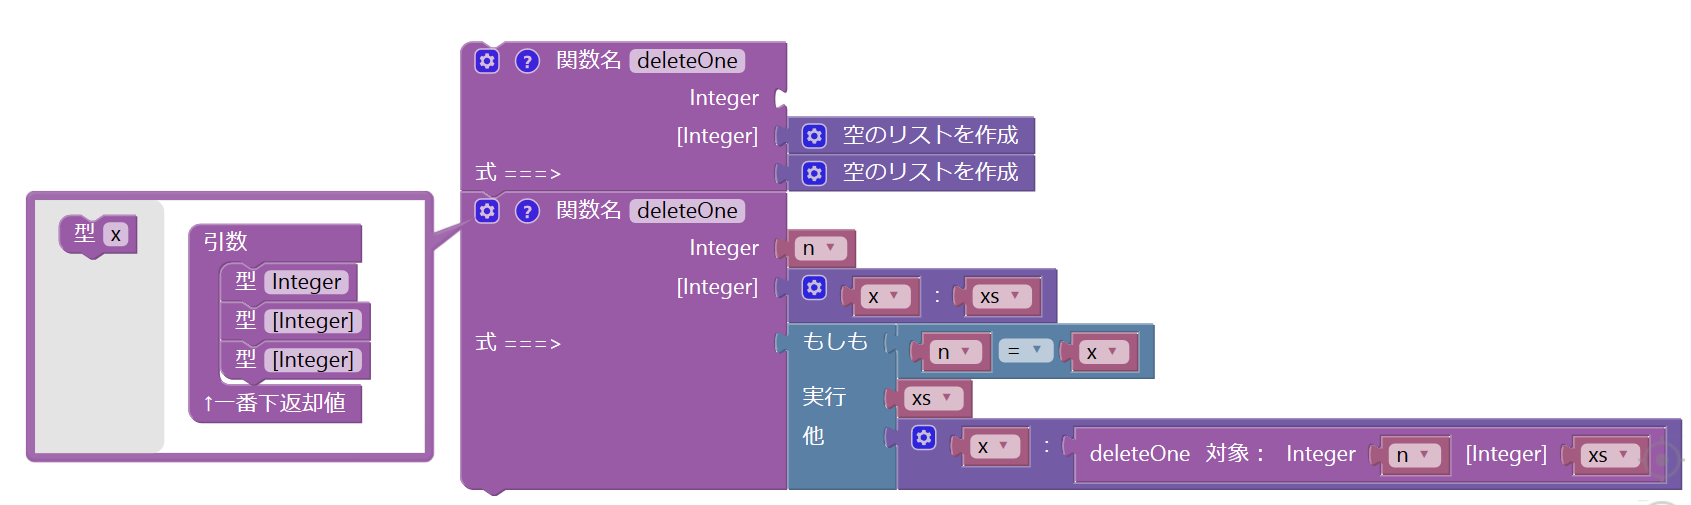
\includegraphics[scale=0.5]{img/haskell_function2.eps}
\caption{関数ブロックと関数呼び出しブロックの接続例}%
\label{fig:haskell_function2}
\end{center}%
\end{figure}% 

\item リストのブロック群

Blockly for Haskell のリストカテゴリーで、内包表記ブロック以外にも新たに3つのリストブロックを実装した。以下の図\ref{fig:haskell_list}に、新たに実装したリストのブロック群のイメージを示す。図中の上のブロックは、リストを表すブロックである。Mutator機能で、小窓の中の項目ブロックを結合コンテナに接続することでリストを表すブロックのソケットを増やすことができる。図中の真ん中のブロックは、リストの中の組を表す。こちらも、上のブロックと同じ要領でソケットを増やすことができる。図中の下のブロックは、リストの値の範囲を表す。いずれのブロックもソケットには、数ブロックや変数ブロックが入る。

\begin{figure}[h]
\begin{center}
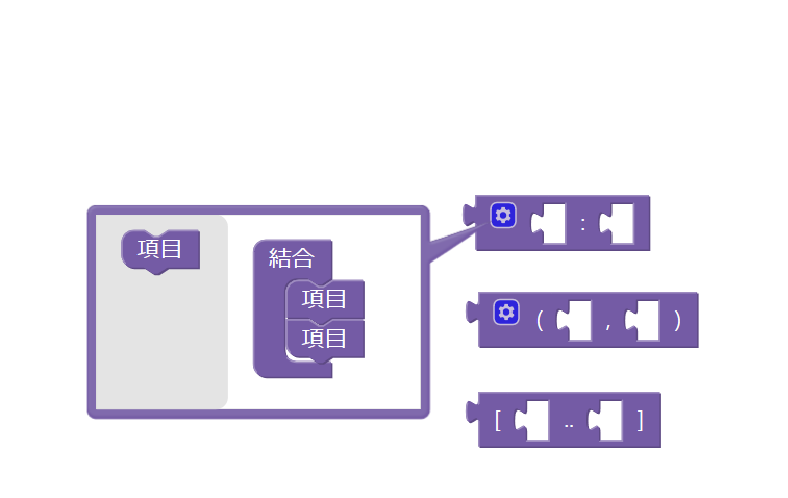
\includegraphics[scale=0.5]{img/haskell_list.eps}
\caption{Haskell のリストブロック群}%
\label{fig:haskell_list}
\end{center}%
\end{figure}% 

\end{itemize} 

   \section{サンプルボタン機能}
Blocklyを初めて使う人にとって、ワークスペース部が何も無い状態でブロックを一から組み立てて、実行できるプログラムを完成させることは難しい。そこで、このシステムの初心者が利用しやすくするためにサンプルボタンを実装した。図\ref{fig:sample}は、サンプルボタンを押したときのワークスペース部のイメージである。WEBページの上部にサンプルボタンを複数個用意した。このサンプルボタンを押すことによって、システム開発者側が用意したブロックを一瞬でワークスペース部に表示される。システム初心者は、その完成されたブロックのプログラムをアレンジしながらシステムを理解することができる。

\begin{figure}[h]
\begin{center}
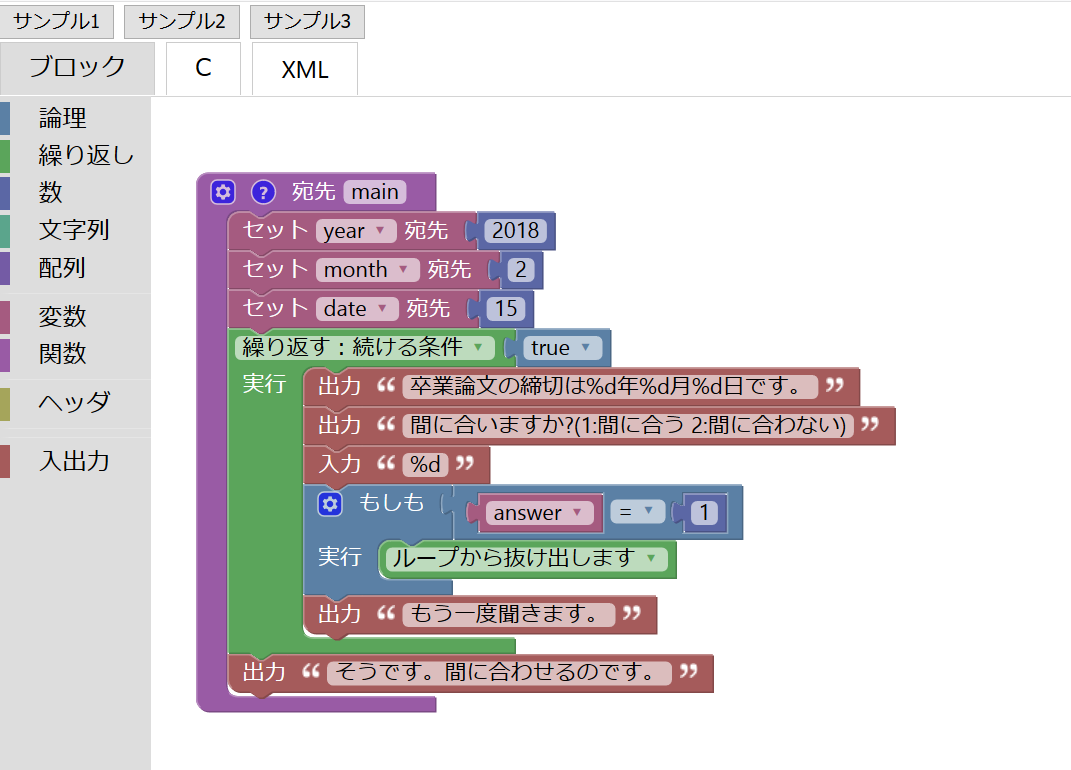
\includegraphics[scale=0.5]{img/sample.eps}
\caption{サンプルボタンを押したときのワークスペース部}%
\label{fig:sample}
\end{center}%
\end{figure}% 

   \subsection{問題点}
   
サンプルボタンを実装したときに問題が発生した。筆者が実装した動的変形機能付きの入出力ブロックがサンプルボタンを押したときに初期状態のままで出力される。つまり、ソケットがない状態でブロックが出力される。入出力ブロックの動的変形機能は、入力フォームの\%の数を検出してソケットの数を増やすのだが、その検出のタイミングが入力フォームに何か変化があるときである。サンプルボタンを押して、入出力ブロックを表示させると入力フォームの変化するタイミングがないため、ソケットも初期状態のままである。

   \subsection{改善点}
   
サンプルボタンの問題点を改善するために、JavaScriptのLocalStorage\cite{LocalStorage}というドキュメントを利用した。LocalStorageとは、データをブラウザ側に保存する仕組みである。同様の有名なドキュメントにCookieがあるが、Cookieには保存の有効期限があるのに対し、LocalStorageには有効期限がない。また、Cookieよりもより多くのデータ量を保存できる。

このLocalStorageを以下のようなソースコードで、入出力ブロックの中の入力フォームの中身を記録することができる。	
関数localStorage.setItemの第1引数に記録させたいブロックのidの属性値、第2引数に記録する入力フォームの中身であり、いずれも文字列である。この記録した中身をサンプルボタンを押した際に、入出力ブロックの入力フォームに渡すことで動的変形を行うことができる。

\shadowbox{
\begin{minipage}[t]{12cm}
\begin{verbatim}
localStorage.setItem(ブロックのidの属性値, 入力フォームの中身); 
\end{verbatim}
\end{minipage}
}


   \section{新たに実装したオプション機能}
   
システムWEBページ上では右上部に5つのボタンが表示されてある。左から、ホーム、ヘルプ、読込み、保存、リセットである。以下の図\ref{fig:option_button}に新たに実装したオプション機能のイメージを示す。

\begin{itemize}

\item ホームボタン

ホームボタンは、筆者が開発したデモページのホームページへ移動できるようになっている。
  
\item ヘルプボタン

ヘルプボタンは、このシステムを初めて使う人向けの機能である。ボタンをクリックすると、順追ってシステムの各機能を説明してくれるようになっている。

\item 読込みボタン

読込みボタンは、過去にBlocklyで保存したプログラムのデータを読込み、ワークスペース部に出力できる機能である。前回に中断したプログラムの続きを行うことができる。

\item 保存ボタン

保存ボタンは、ワークスペース部で組み立てたプログラムを保存することができる。保存形式は、XMLである。プログラムを保存しておけば、次回Blocklyを立ち上げたときに、プログラムの続きから行うことができる。

\item リセットボタン

リセットボタンは、ワークスペース部で組み立てたプログラムをリセットして何もない状態から再開できるボタンである。このボタンをクリックする前に、組み立てたプログラムを一旦、保存しておくことを推奨する。

\end{itemize} 

\begin{figure}[h]
\begin{center}

\includegraphics[scale=0.5]{img/option_button.eps}
\caption{新たに実装したオプション機能}%
\label{fig:option_button}
\end{center}%
\end{figure}% 



   \chapter{評価}
   
香川研究室の学部生3名と院生2名を対象に、本システムの評価を行った。本章では、システム評価について述べる。
   
   \section{項目}
   
実際にシステムを使用してもらい、その後以下の評価項目に自由に回答する形式で行った。

\begin{itemize}
\item 操作方法は直感的に分かったか
\item 使ったブロックとそのブロックの評価
\item 欲しい機能やブロック
\item 不具合報告(無ければ書かなくてよい)
\end{itemize} 
   
   \section{結果}

学部生3名には Blockly for C を、院生2名には Blockly for Haskell について評価してもらった。
Blockly for JavaScript は、既存のGoogleが実装したシステムでも完成度が高く、本研究ではほとんど手を加えなかったため評価対象から外した。Blockly for Flex は、尾崎の先行研究から正規表現ブロックに動的変形機能を適用させることができなかったため、評価対象から外した。
評価の結果、それぞれのシステムの評価項目で次のような意見が挙がった。

   \subsection{Blocly for C を利用しての意見}
   
Blockly for C では、全体的にシステムに関して肯定的な意見が多くみられた。特に、動的変形機能を適用させた入出力ブロックはとても評判が良かった。しかし、その動的変形機能にも一部不具合や例外処理に適応できておらず、まだまだ改善の余地もあることが判明した。以下は、評価項目での具体的な意見である。
   
\begin{itemize}
\item 操作方法は直感的に分かったか

    - 選択中のブロックが枠線で強調されたため、何かしらの動作ができることが分かり、操作する際の足がかりとなり良かった

    - ブロックにマウスカーソルを合わせるとブロックの詳細説明が表示され、分かりやすかった

    - 関数の引数名に重複がある場合、知らせてくれるのが良いと思った

    - 取り外しのできないブロックの色が薄く表示されており、着脱可能かどうか分かりやすかった
    
    - 直感的にわかったが、配列などの項目の設定などは一回使わないとわかりづらい

\item 使ったブロックとそのブロックの評価

 - 出力ブロック: \%で出力変数を動的に変更できるのは良いと思った

 - 文字'\%'を出力する際には、C言語で"\%\%"と入力する必要があるが、この場合でも出力変数用の\%として認識されていたため、'\%'の出力ができないと思った

\item 欲しい機能やブロック

    - 文字列や実数の変数ブロック

    - 引数名重複エラーなどのエラーマークは青ではなく、赤に近い色が良いと思う
    
    - ブラウザにある戻る進むのような機能は欲しいなと感じた
    
    - ビット演算のブロックはあっても良いかなと感じた

\item 不具合報告(無ければ書かなくてよい)

    - 不具合ではないのですが、サンプル1の出力ブロックは\%による変数の動的検出のないブロックなのですが、動的検出のあるブロックと判別がつかないため、ブロックの見た目で判断できるようにしたほうが良いと思う

    - サンプル3の"卒業論文の締切は\%d年\%d月\%d日です。"を出力するブロックの変数(year、month、day)がセットされていない
    
\end{itemize} 

   \subsection{Blocly for Haskell を利用しての意見}
   
一方でBlockly for Haskell では、評価の際に操作はできたものの分からない点や改善案が多く見られた。また、不具合も多く他の言語のシステムでも共通するような不具合も本システムで発見された。Blockly for Haskell に関しては、まだまだ表現できるプログラムが限定的で、本システムで実装したブロックでも改善点が多いので、まだまだ未熟なシステムであることが痛感される結果となった。以下は、評価項目での具体的な意見である。
   
\begin{itemize}
\item 操作方法は直感的に分かったか

- Blocklyを触ったのは初めてでなかったのもあるが、普通に操作できたと思う

- どういう風につなげて良いかとかどう関数を作ったらいいかとかがわからなかった

\item 使ったブロックとそのブロックの評価

- 関数のブロック作成が分かりづらく感じた。
実際に関数を作成しようとすると、どうしてもブロックの数が増えるのは少し面倒に感じた

\item 欲しい機能やブロック

- 関数のブロックの扱いが分かりづらかったので、その説明または使いやすいブロックになるといいと思った

- letをdoを使わずに関数で使いたい

- Haskellの授業の序盤の補助としてシステムの使用を考えるなら、ある程度出す問題に沿ったまとまったブロックをあらかじめ作成するのがいいのではないかと思った

\item 不具合報告(無ければ書かなくてよい)

- 変数のところにある変更aは変数aではないか?

- 関数を呼び出す時に変数をn-1みたいな感じでやったらかっこがついてなかった

- 自分がやるとサンプルが出なかった。(win8.1 クローム最新)

- 関数で式が2つになったり引数部が上にきたりするときがあり、式2つになったときもHaskellのコードをみたら1つだけだった

- スクロールが必要なほどブロックの数が多いタブは一番下のブロックが半分ほど隠れてしまう(デフォルトから2段階小さくすれば表示可能になる)

\end{itemize}
   \chapter{おわりに}
   
   \section{まとめ}
   
大学の講義で学習する言語に対応させるために、WebベースグラフィカルプログラミングエディタBlocklyの多言語対応を行った。その際に、ブロックの種類が多くなりすぎないようにMutator以外の動的変形の機能の拡張も行った。この拡張によって、柔軟性のあるプログラミンング言語をブロックの形状によって制限されないようになっている。また、拡張した機能もシンプルで、学習者の負担も増やさないようにしている。これらの特徴は、第1章で述べたシステムに求められる

\begin{itemize}
\item システムの操作が容易
\item 大学の講義で学習する言語に対応させるための多言語化
\item プログラミング言語の柔軟性の保持
\end{itemize} 

という要件を目指したものである。
しかし、実際に授業で使用してもらっていないので、今回の研究室で得られたフィードバックをもとにシステムを改良し、授業で効果を確認する必要がある。
   
   \section{今後の課題}
   
大学の授業で効果を確認できるようなシステムを目指すために、以下に本システムの課題を述べる。
   
\begin{itemize}

\item Blockly の対応言語をもっと増やす

本システムでのBlocklyの対応言語は、C、JavaScript、Haskell、Flex の4種類にとどまった。それぞれの対応言語は種類や用途がまったく違うプログラミング言語である。これらの言語は、いずれも本大学の講義で学ぶ言語であるが、本システムの対応言語が大学の講義で学ぶ言語にすべて対応できているとはいえない。そこで、この目標に達するために次の対応言語として、Java、Ruby、htmlの実装が必要である。

\item Blockly for C の配列に対応させる

本システムの Blockly for C には、配列に対応させることができなかった。Blockly for JavaScript では、既存のシステムでリストが対応しており、Blockly for Haskell のリストは本システムで初めて実装した。これらを参考にしながら、Blockly for C の配列に対応させる必要がある。

\item Blockly for Haskell の汎用性を増やす

本システムの Blockly for Haskell は、大学の講義に対応したシステムにするために本学科での講義「プログラミンング・パラダイム」の内容に沿って作成した。しかし、講義の内容すべて対応させることはできず、本システムは限定的なものとなってしまった。そこで、Blockly for Haskell の汎用性を増やすために、代数的データ型、クラス宣言、インスタンス宣言にも対応させる必要がある。

\item Blockly for Flex に本システムで開発した動的変形を適用させる

先行研究の Blockly for Flex では、範囲の任意の文字を表す正規表現ブロックが実装されていた。しかし、このブロックは単体での範囲しか表すことができず、ソケット付きのブロックと新たに正規表現ブロックを追加しても2つの範囲が限界である。そこで、3つ以上の文字範囲を表すことができるように、本システムの Blockly for C で実装した入出力ブロックの動的変形機能をこの正規表現ブロックに適用させる必要がある。以下の図\ref{fig:flex_dynamic_deformation}に、動的変形機能を正規表現ブロックに適用したイメージを示す。

\begin{figure}[h]
\begin{center}
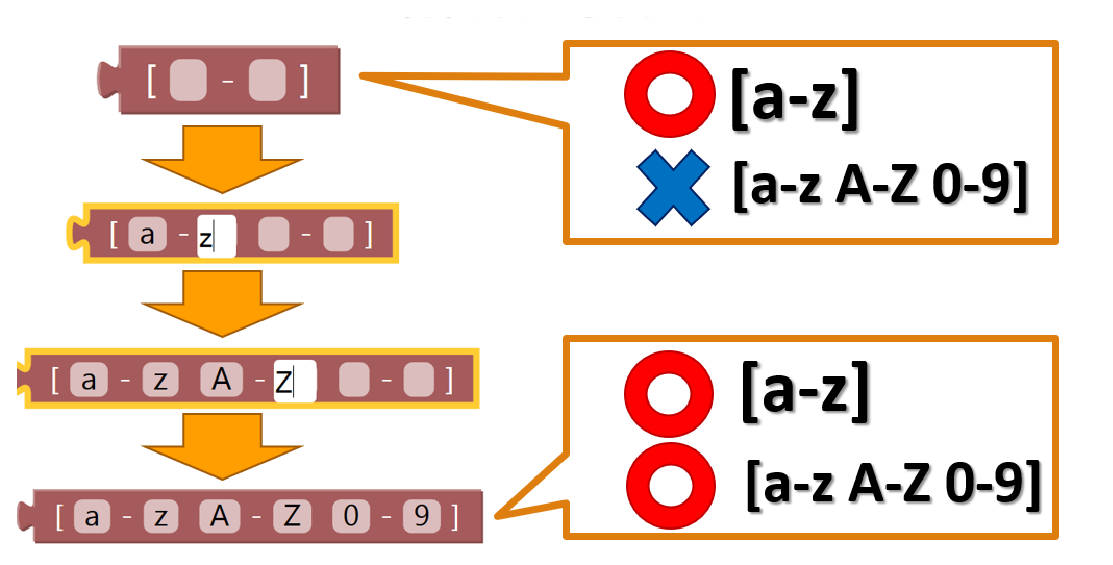
\includegraphics[scale=0.5]{img/flex_dynamic_deformation.eps}
\caption{動的変形機能を正規表現ブロックに適用したイメージ}%
\label{fig:flex_dynamic_deformation}
\end{center}%
\end{figure}% 

\item 実行タブの実装

本システムの評価の際に、「このプログラムをシステム上で実行するにはどうすればよいか」といった質問があった。本システムでは、プログラムを実行する機能は実装できていない。しかし、本研究室がオープンキャンパスの際に展示するBlocklyを使ったお絵かきプログラミングには、プログラムを実行する機能が実装されている。本システムでも、実行できる機能を追加しなければならない。

\item ブロック接続部の改善

本システムの Blockly for Flex で接続できないブロックがある。内包表記ブロックの限定式のところで、直接式ブロックを接続しようとしても、接続の形状的に接続することができない。そこで、急遽、接続できないときのために作られたブロックを用意した。以下の図\ref{fig:connection_bug}の黒色のブロックが急遽、用意したブロックである。このブロックは、プログラム上では何も意味を持たないものであり、このブロックがワークスペース部にある状態で、XMLコードタブを押しワークスペース部に戻るとエラーでプログラムが出力できなくなる。この問題を解決するためにも、ブロックの接続部の改善を検討しなければならない。

\begin{figure}[h]
\begin{center}
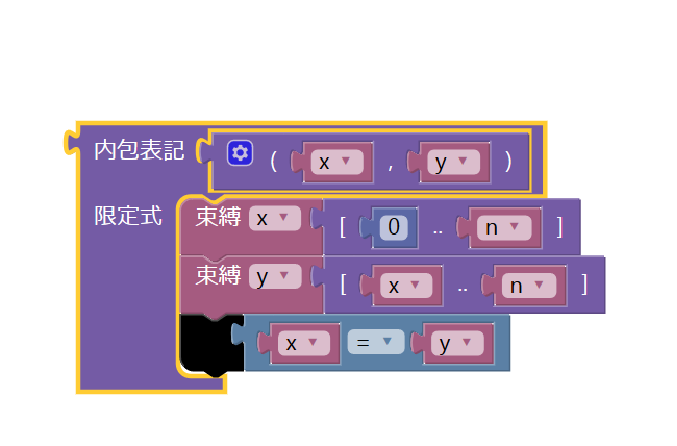
\includegraphics[scale=0.5]{img/connection_bug.eps}
\caption{接続できないときのために作られたブロックのプログラム例}%
\label{fig:connection_bug}
\end{center}%
\end{figure}% 

\end{itemize} 
 

\acknowledgment  % 謝辞

本研究においてご指導を承りました香川考司先生に心からの感謝の意を表します。

また、システムの評価に協力して頂いた、大橋健太さん、仁科陽彦さん、朝野有也さん、伊藤拓海さん、太田圭祐さんに深く感謝します。

\begin{thebibliography}{99} % 参考文献
                                  
  \bibitem{Blockly} % 論文
 Google 
 ``Blockly'', https://developers.google.com/blockly/, 2018年2月14日閲覧.

  \bibitem{ozaki} % 論文
 尾崎陽一,
 ``Webベースグラフィカルプログラミングエディタを用いた円滑な移行が可能なC言語学習支援環境の開発'', 香川大学大学院工学研究科信頼性情報システム工学専攻 2014年度修士論文, 2015年.
 
  \bibitem{yamagata} % 論文
 山形悠人
 ``WEBベースグラフィカルプログラミングエディタを用いたC言語学習支援への問題提示機能の実装'', 香川大学工学部電子・情報工学科2016年度卒業論文, 2017年.
 
  \bibitem{LocalStorage} % 論文
HTML Standard, https://html.spec.whatwg.org/multipage/webstorage.html, 2018年2月14日閲覧.
 

\end{thebibliography}



\insertindex % 索引を出力                                 
\printindex
  
\end{document}
